\documentclass[11pt]{article}

\usepackage[lofdepth,lotdepth]{subfig}
\usepackage{graphicx}
\usepackage{fancyhdr}
\usepackage{amsmath,amssymb}
\usepackage[small,compact]{titlesec}
\usepackage{floatflt}
\usepackage{fullpage}
\usepackage{xcolor}

%\setlength{\textwidth}{6.5in}
%\setlength{\leftmargin}{0.5in}

\begin{document}

\begin{center}
\bf Preliminary Baseline Design (v1) Sensitivity Modeling \\
J. Ruhl, I. Gullett\\
5/14/2021
\end{center}

\section{Introduction}

This note describes the investigation of PBDR\_v1 sensitivity modeling, including the impact of varying representative input parameters.  
We use bolo-calc as the calculation engine for these investigations.

The model starts with a prescription for the optical components of each telescope, including losses and temperatures of each component.  These, along with a band specification and atmospheric emission profile specified by the site, elevation pointing, and precipitable water vapor (pwv), are used to calculate the optical loading on the detector.

That optical loading is used to set the target saturation power of the detectors in each band, for each telescope.  Those, plus some additional input parameters, are used to calculate the per-detector NETs.  

The inputs for each telescope are in the associated yaml files.  In this iteration we are using square (flat) detector bandpasses, which are designed to approximate the centers and widths of those designed by Jeff McMahon for Act/SO.


\section{Baseline Results}

Insert tables of $P_{optical}$, $P_{sat}$, NEPs (photon, detector, and total) and NETs.


\section{Parameter Variations}

Varying a single input parameter at a time tells us how strongly it affects any outputs of interest.  We are mostly interested in 
$P_{optical}$ and the NET.   For each such study, we need to decide whether we are holding any other parameters constant;  
for example, when varying the $T_c$, we can either have it affect $P_{sat}$, or keep $P_{sat}$ constant.   The former is relevant if we are asking about how $T_c$ impacts sensitivity for a detector that is already built, while the latter tells us how $T_c$ impacts sensitivity if haven't
built the detector yet and can design the leg lengths and/or cross-sections to keep $P_{sat}$ constant.

\begin{figure}[p]
         \centering
         \subfloat[Subfigure 1 list of figures text][CHLAT]{
             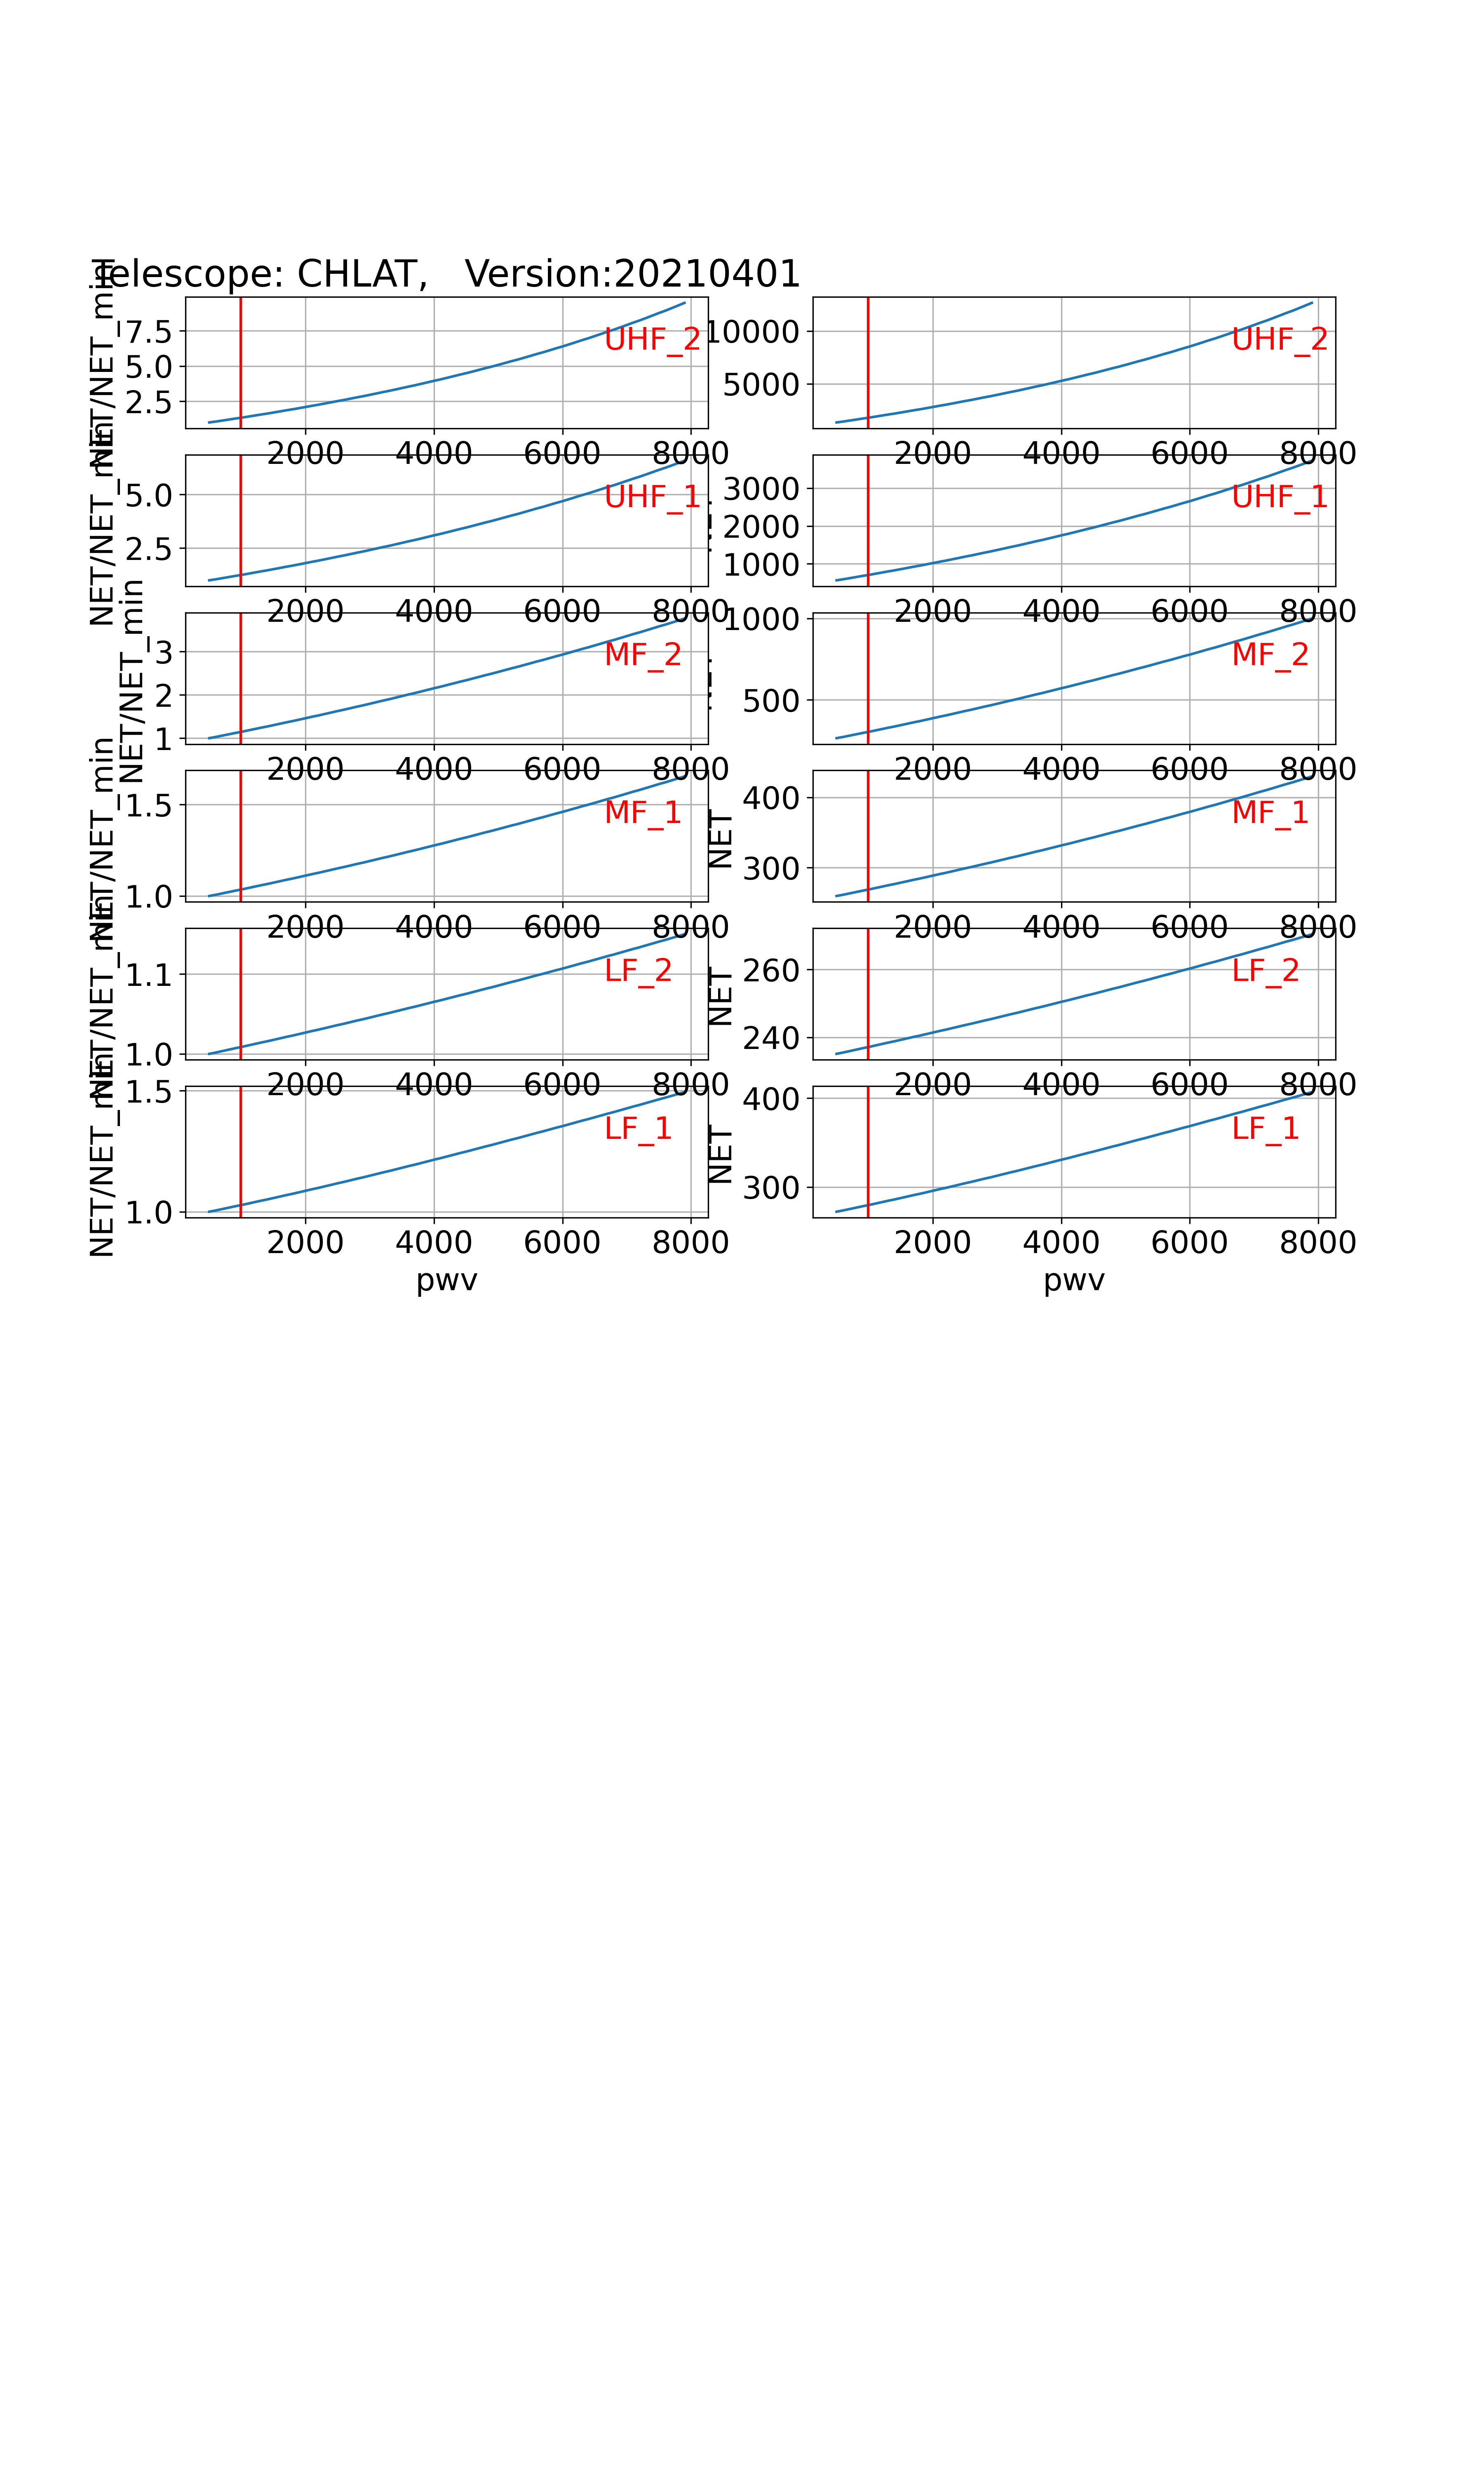
\includegraphics[width=0.33\textwidth]{plots/CHLAT_20210401_NET_v_pwv.png}
             %\caption{}
         }
     %\hfil
        \subfloat[Subfigure 1 list of figures text][SPLAT]{
           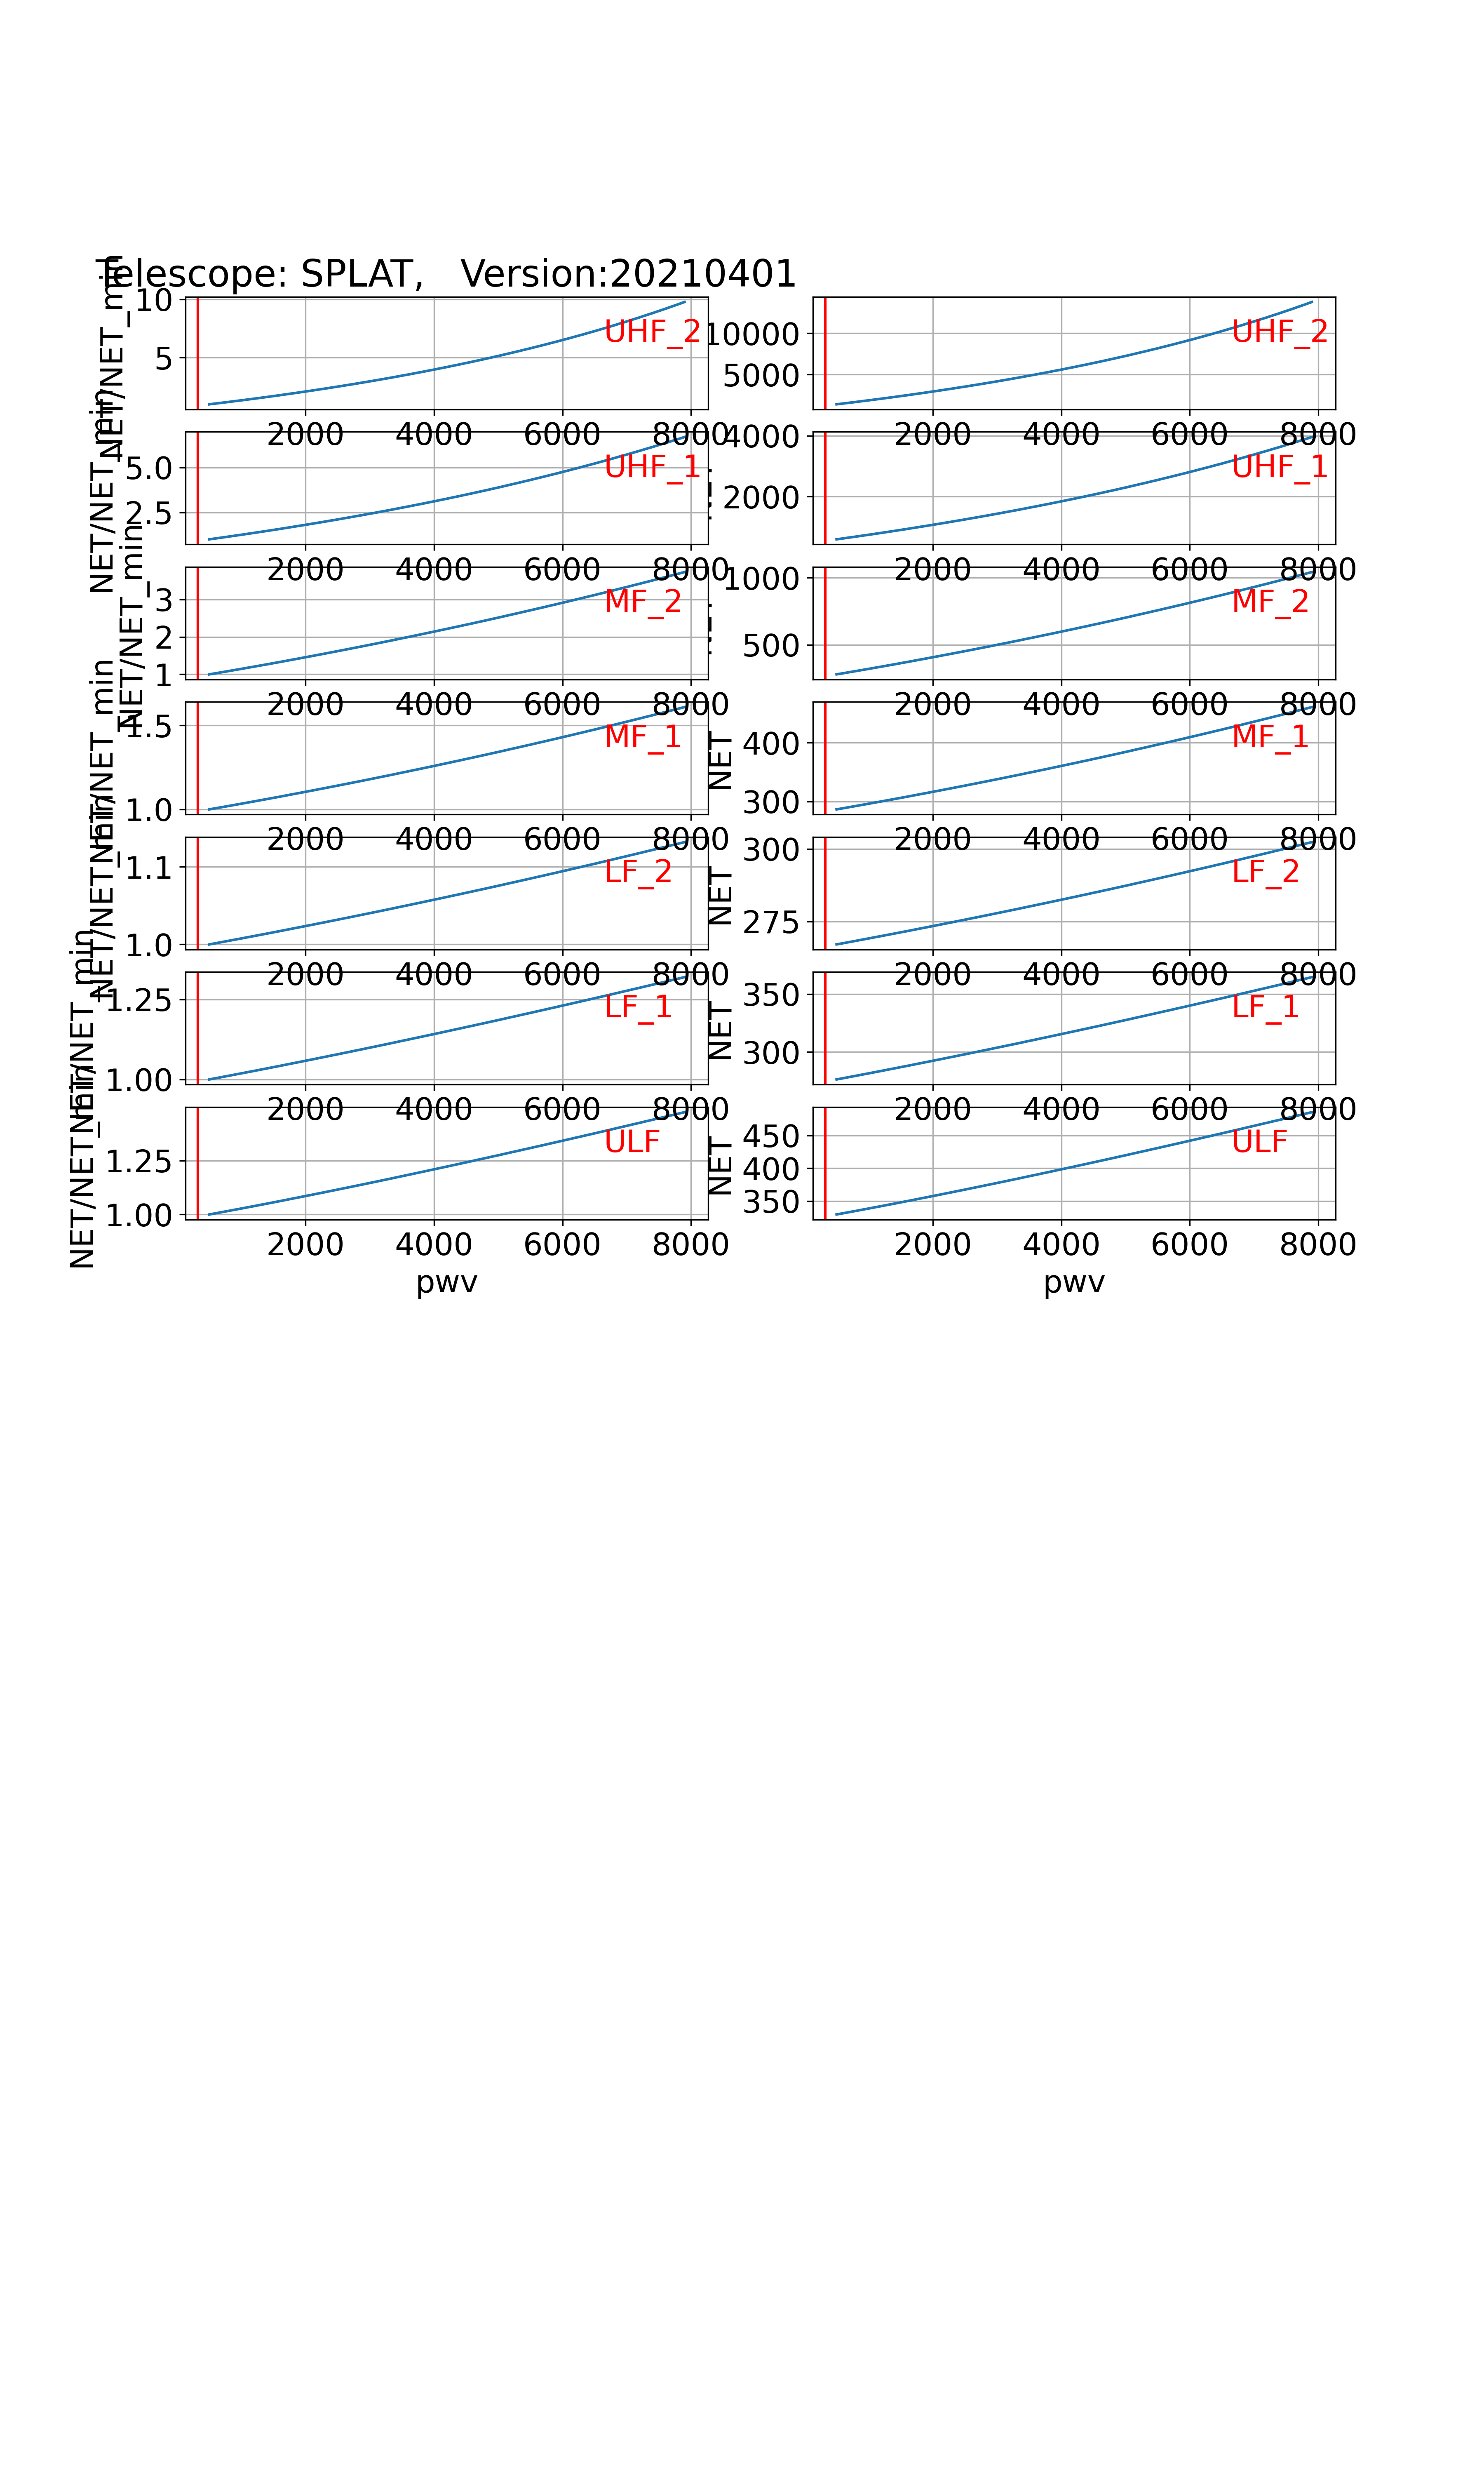
\includegraphics[width=0.33\textwidth]{plots/SPLAT_20210401_NET_v_pwv.png}
           %\caption{}
        }    
        \subfloat[Subfigure 1 list of figures text][SAT]{
            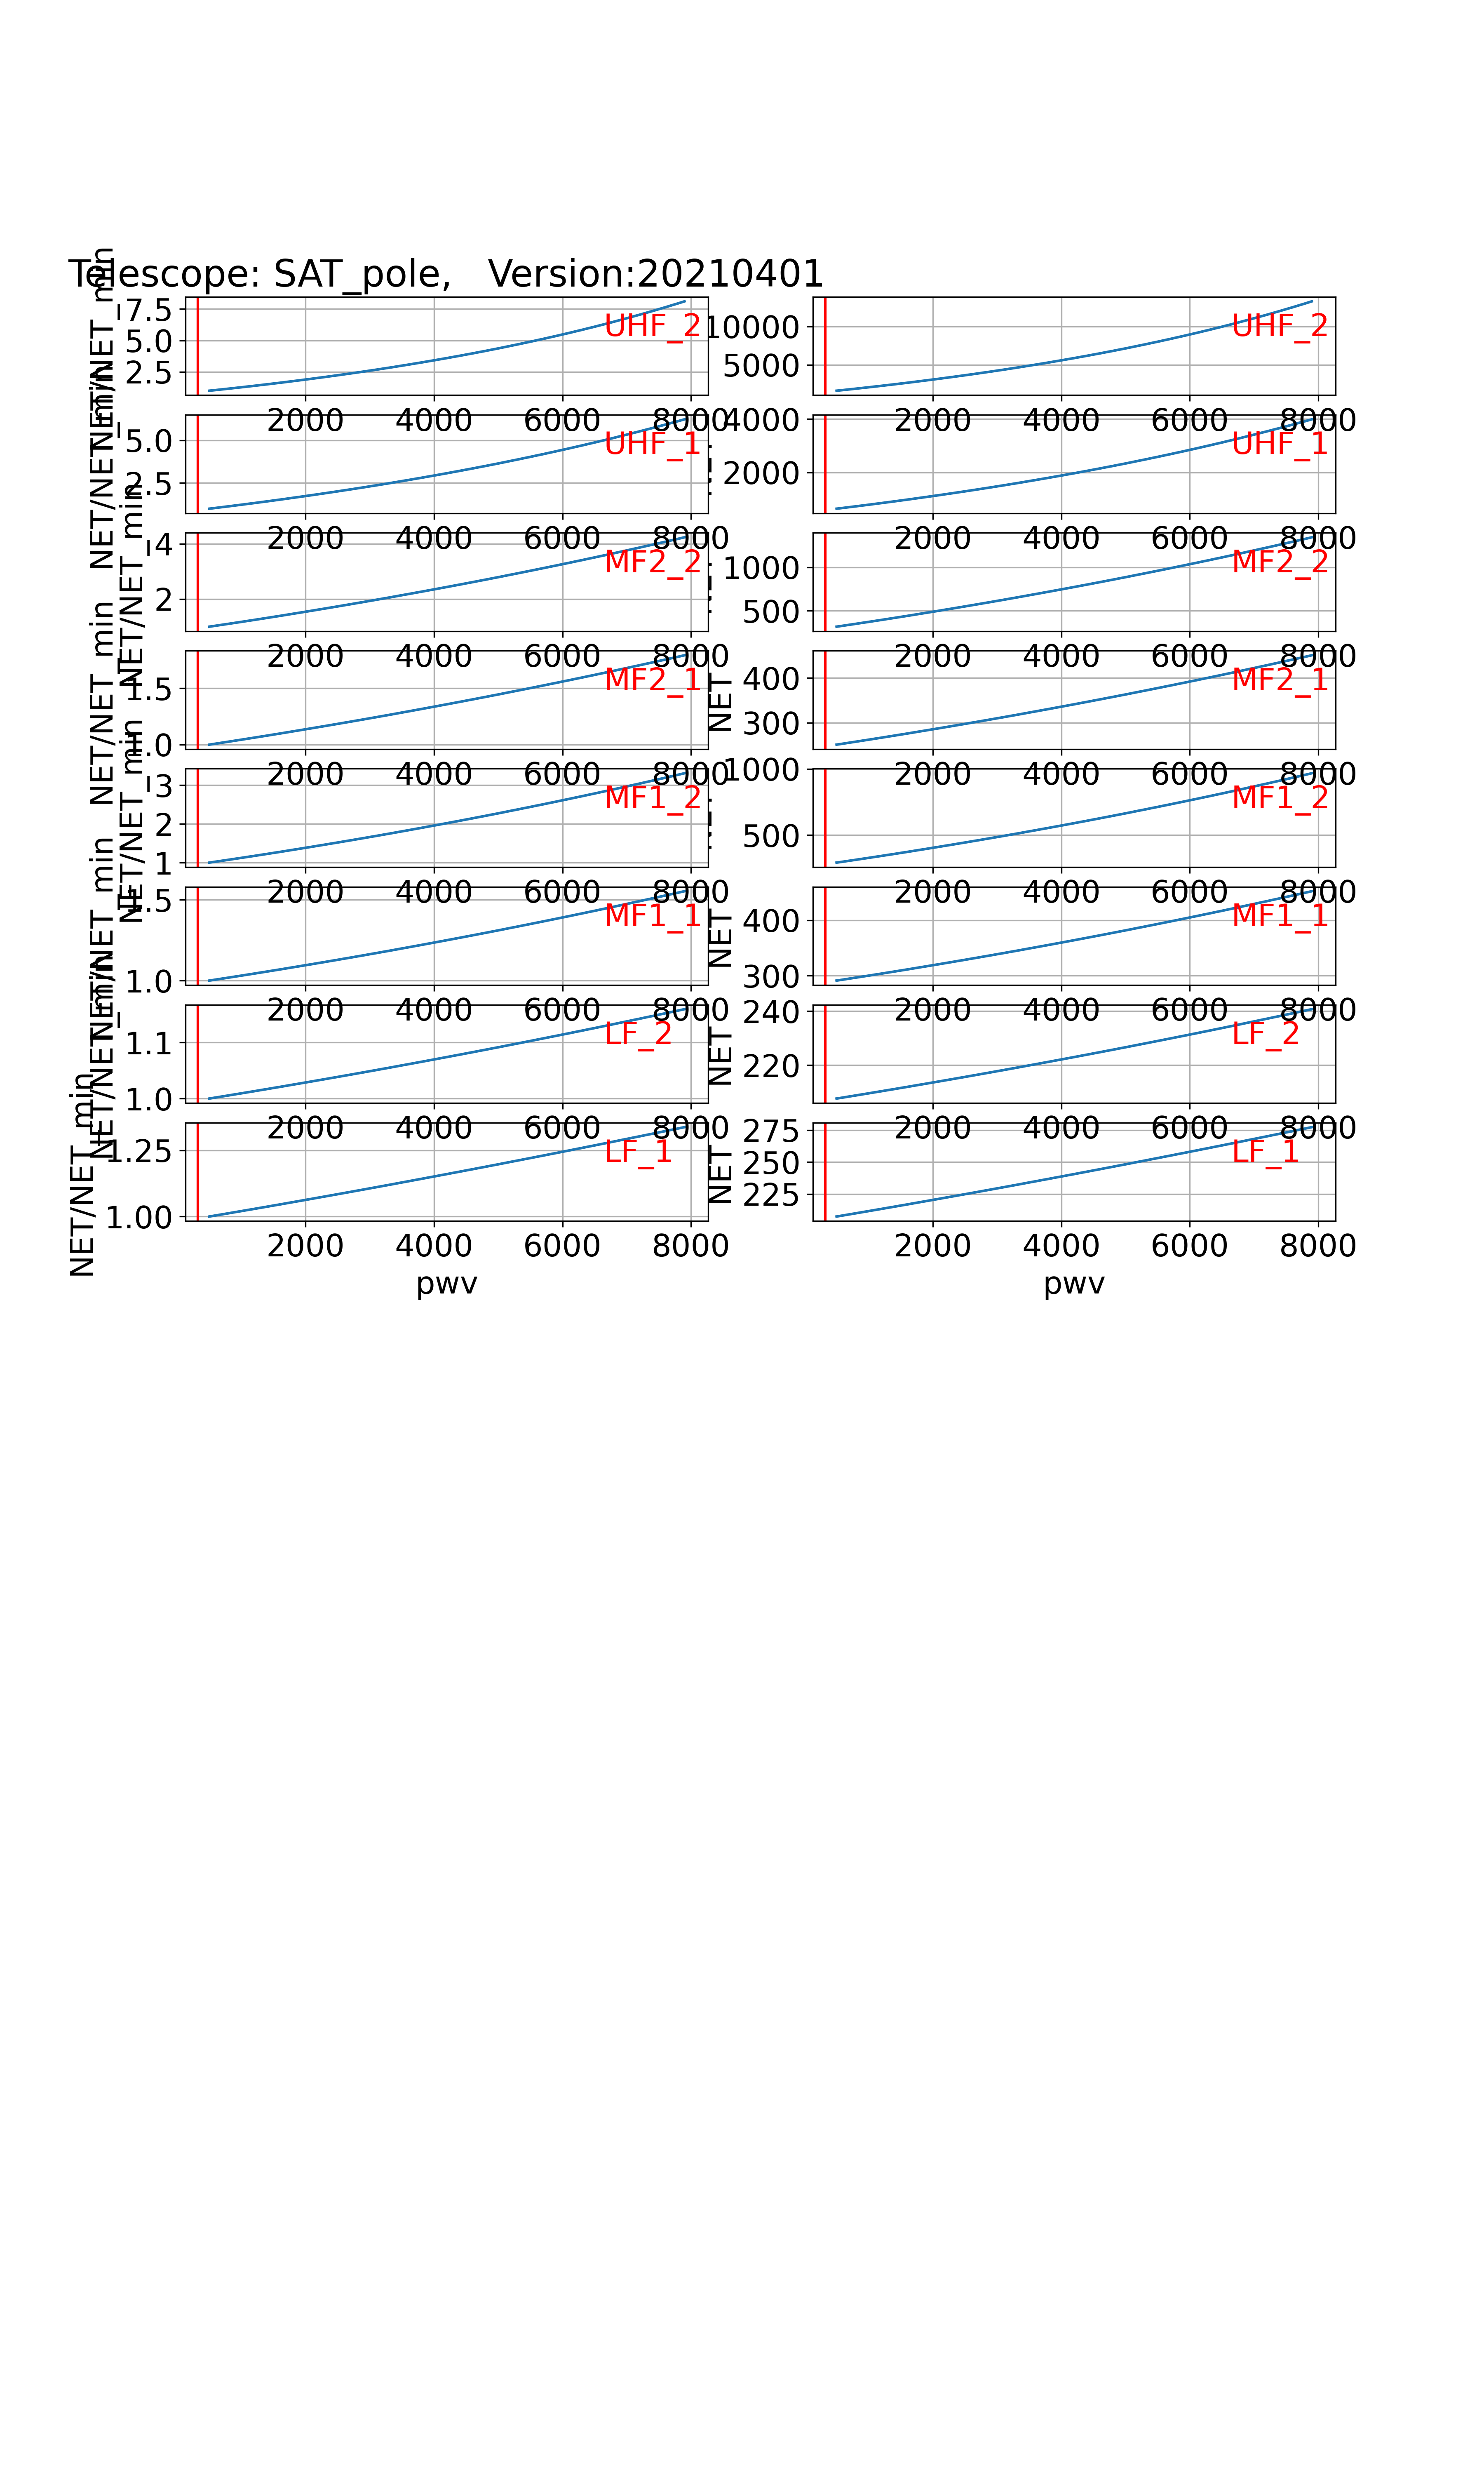
\includegraphics[width=0.33\textwidth]{plots/SAT_pole_20210401_NET_v_pwv.png}
            %\caption{}
        }
     %\vspace{-2\baselineskip}
     \caption{NET vs PWV}
     \label{fig:PWV}
\end{figure} 

\begin{figure}[p]
         \centering
         \subfloat[Subfigure 1 list of figures text][CHLAT]{
             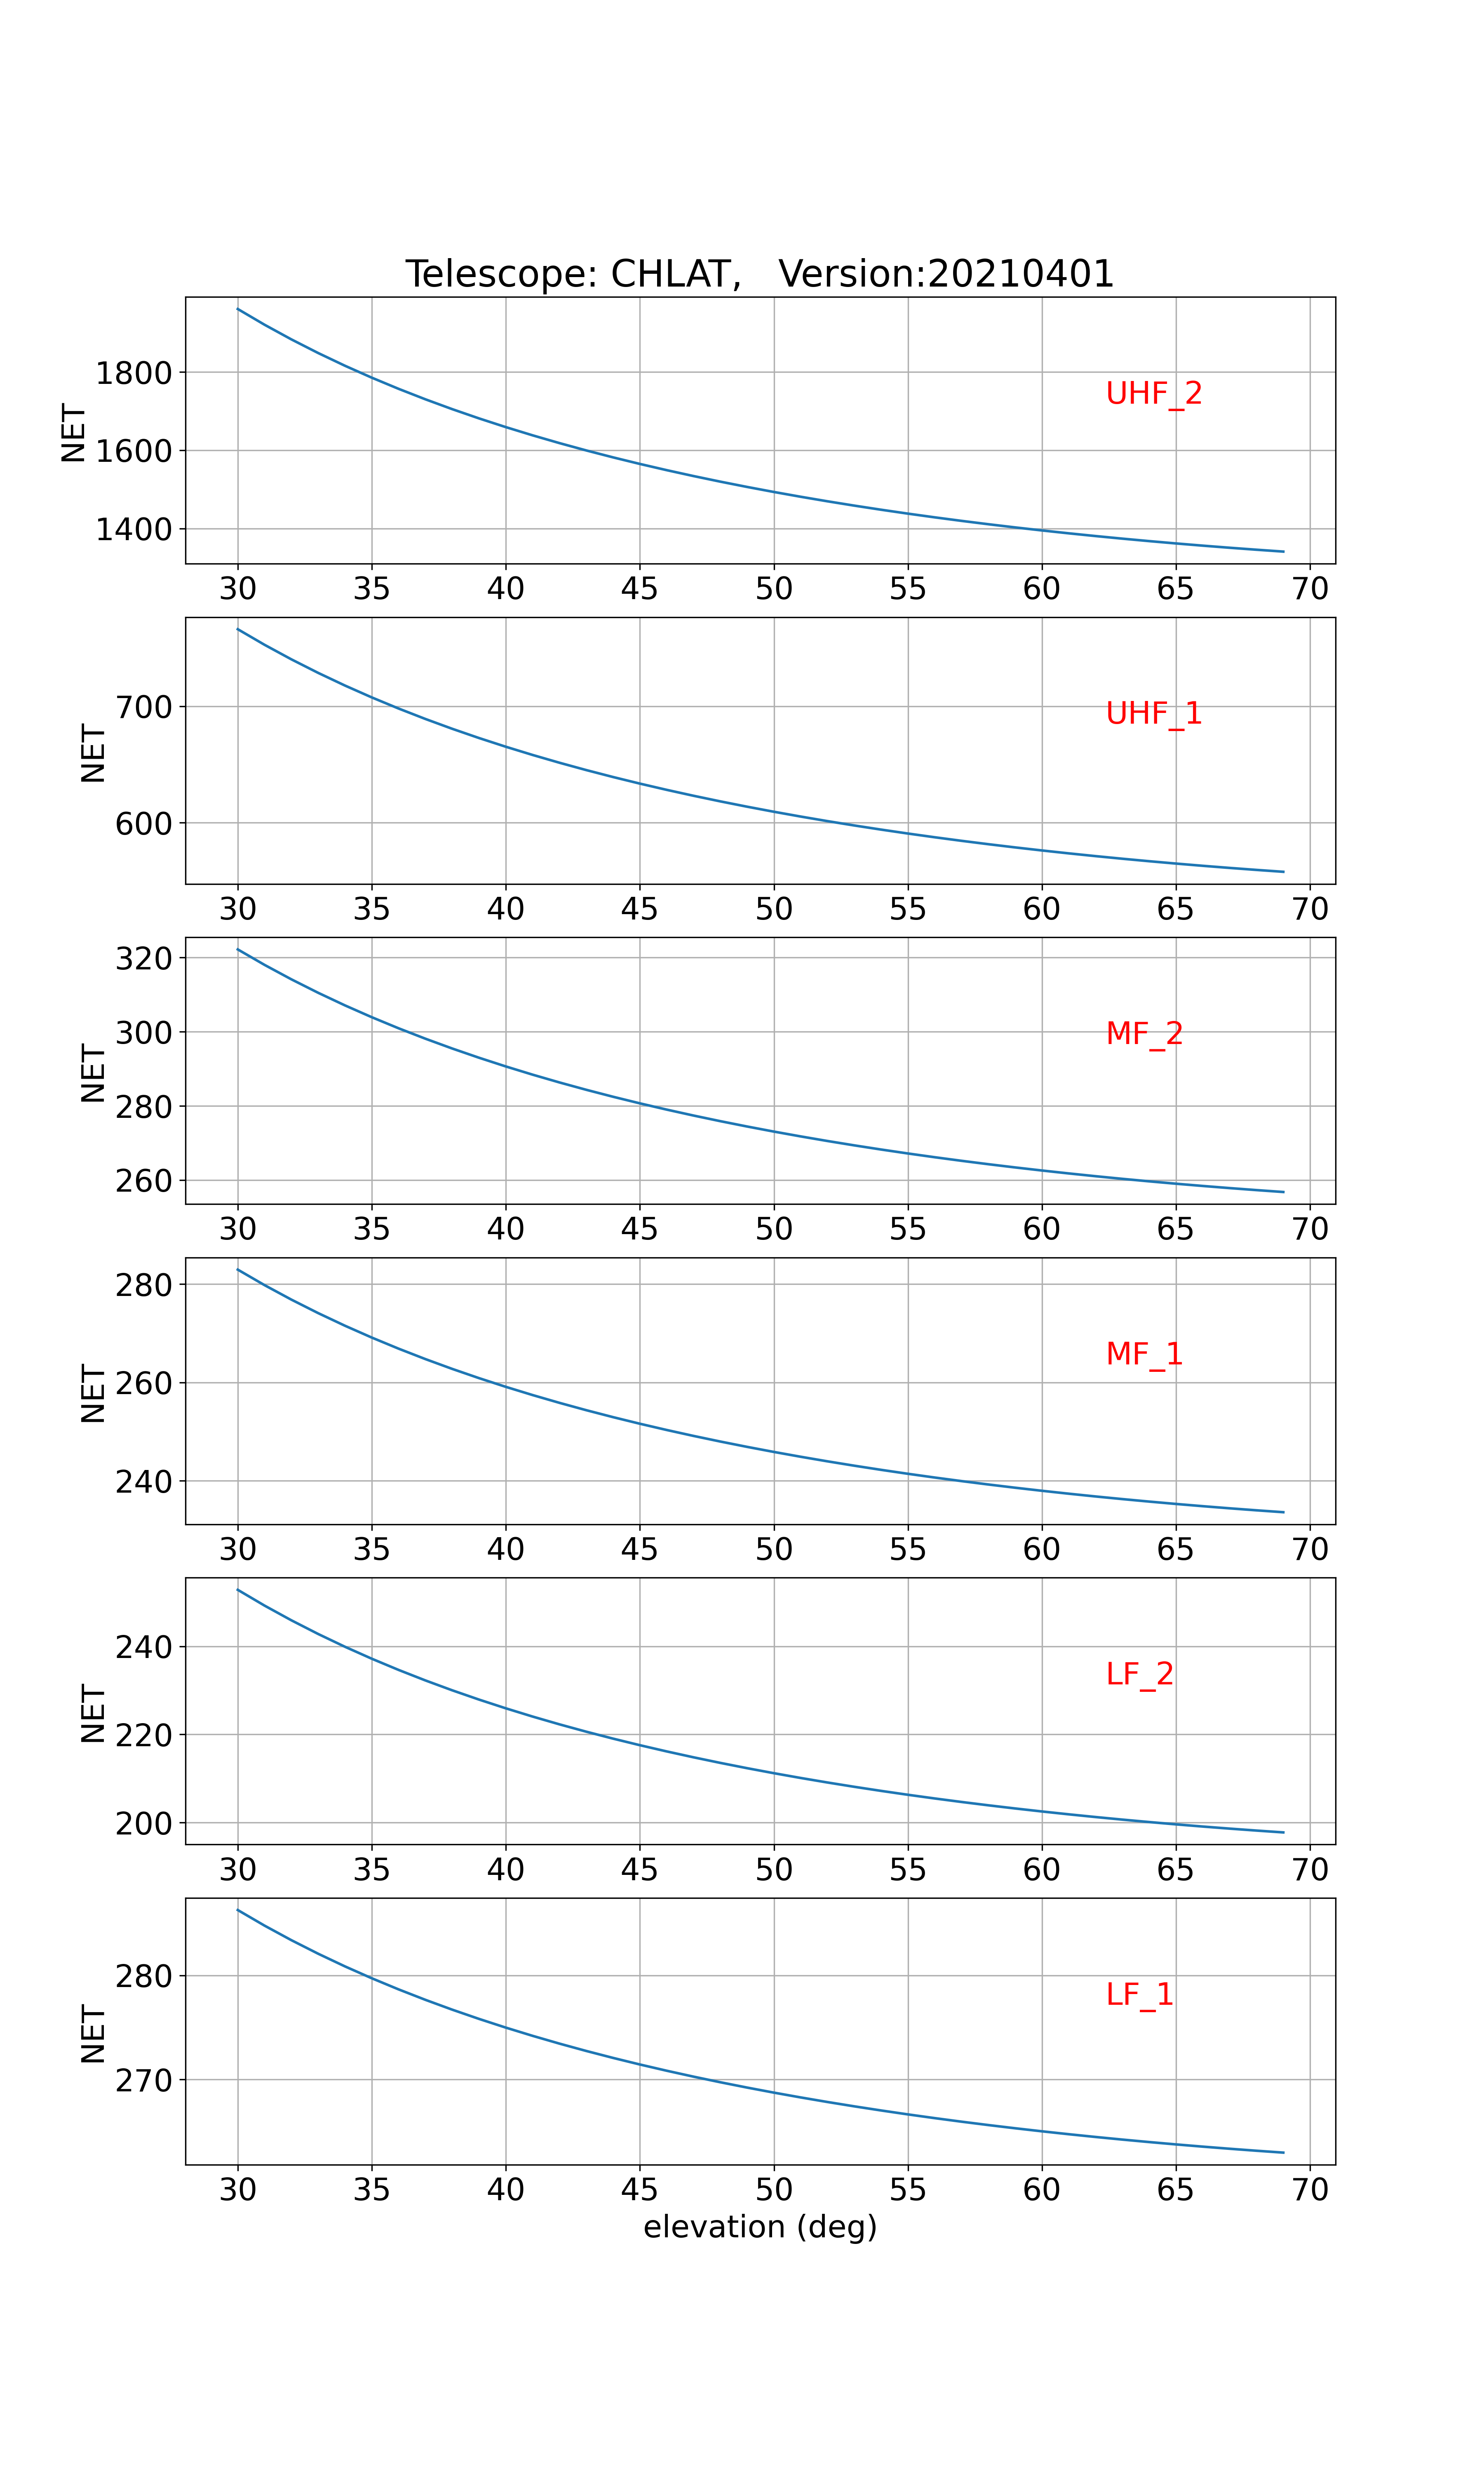
\includegraphics[width=0.33\textwidth]{plots/CHLAT_20210401_NET_v_elevation.png}
             %\caption{}
         }
     %\hfil
        \subfloat[Subfigure 1 list of figures text][SPLAT]{
           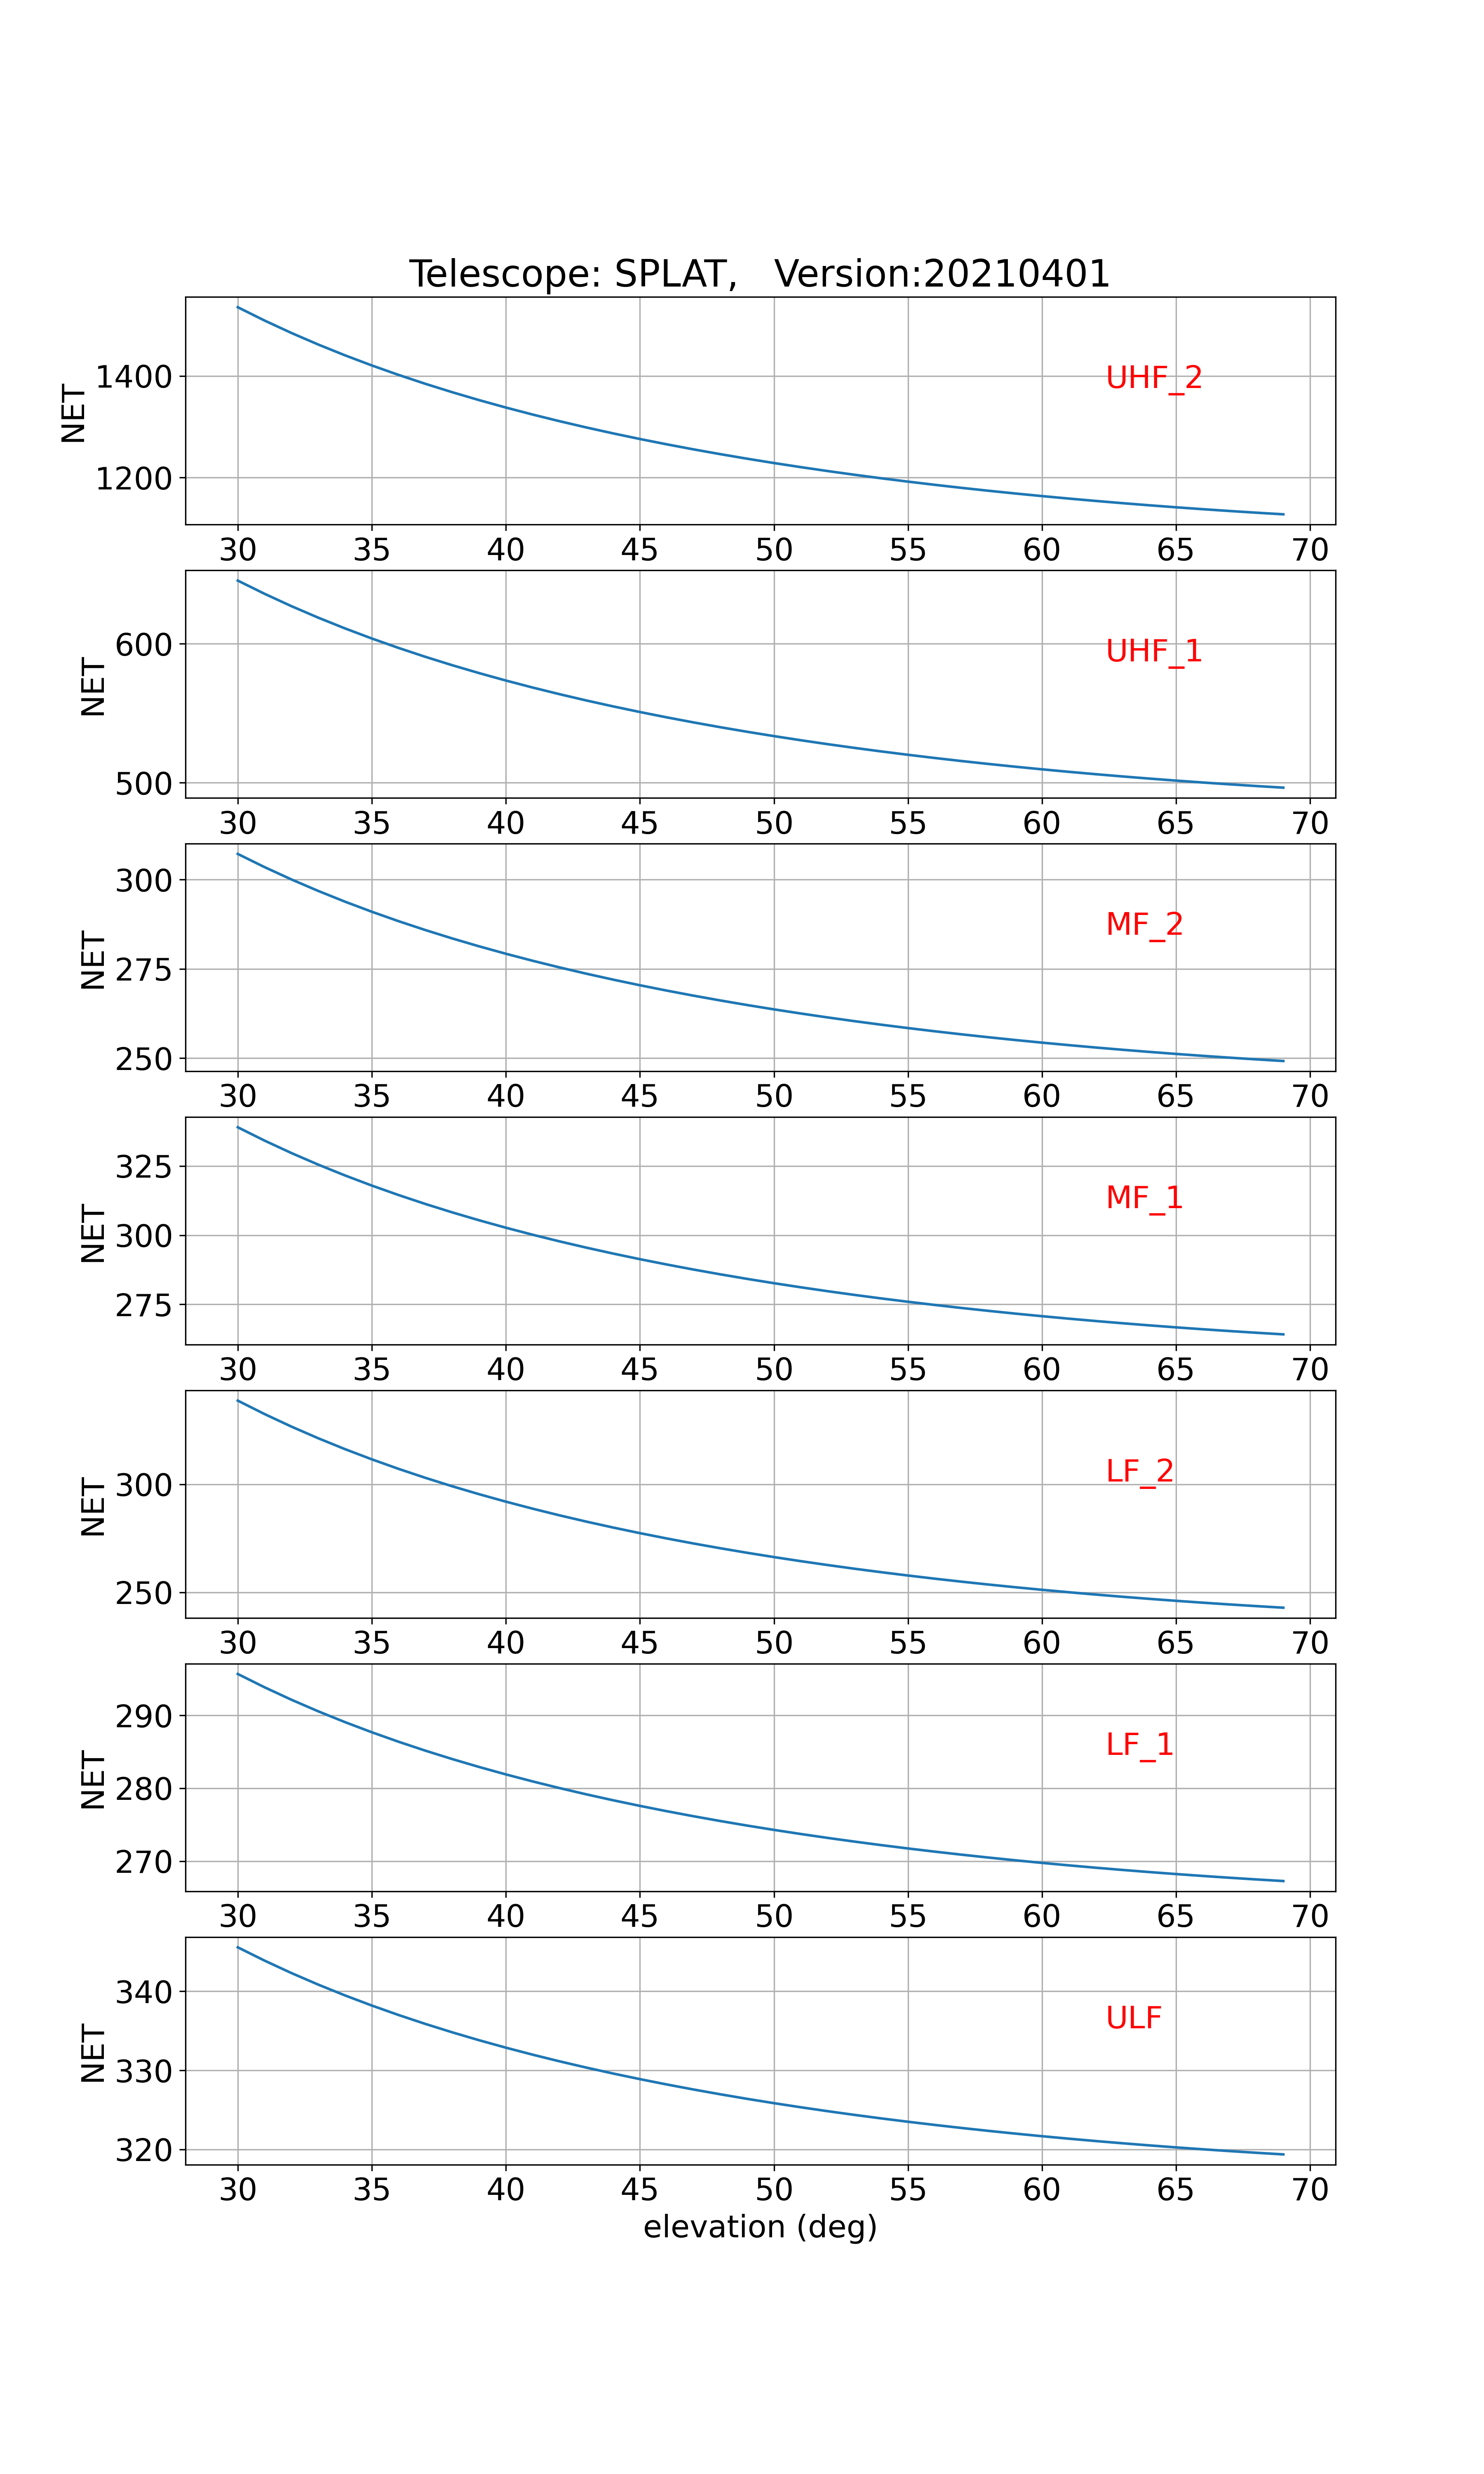
\includegraphics[width=0.33\textwidth]{plots/SPLAT_20210401_NET_v_elevation.png}
           %\caption{}
        }    
        \subfloat[Subfigure 1 list of figures text][SAT]{
            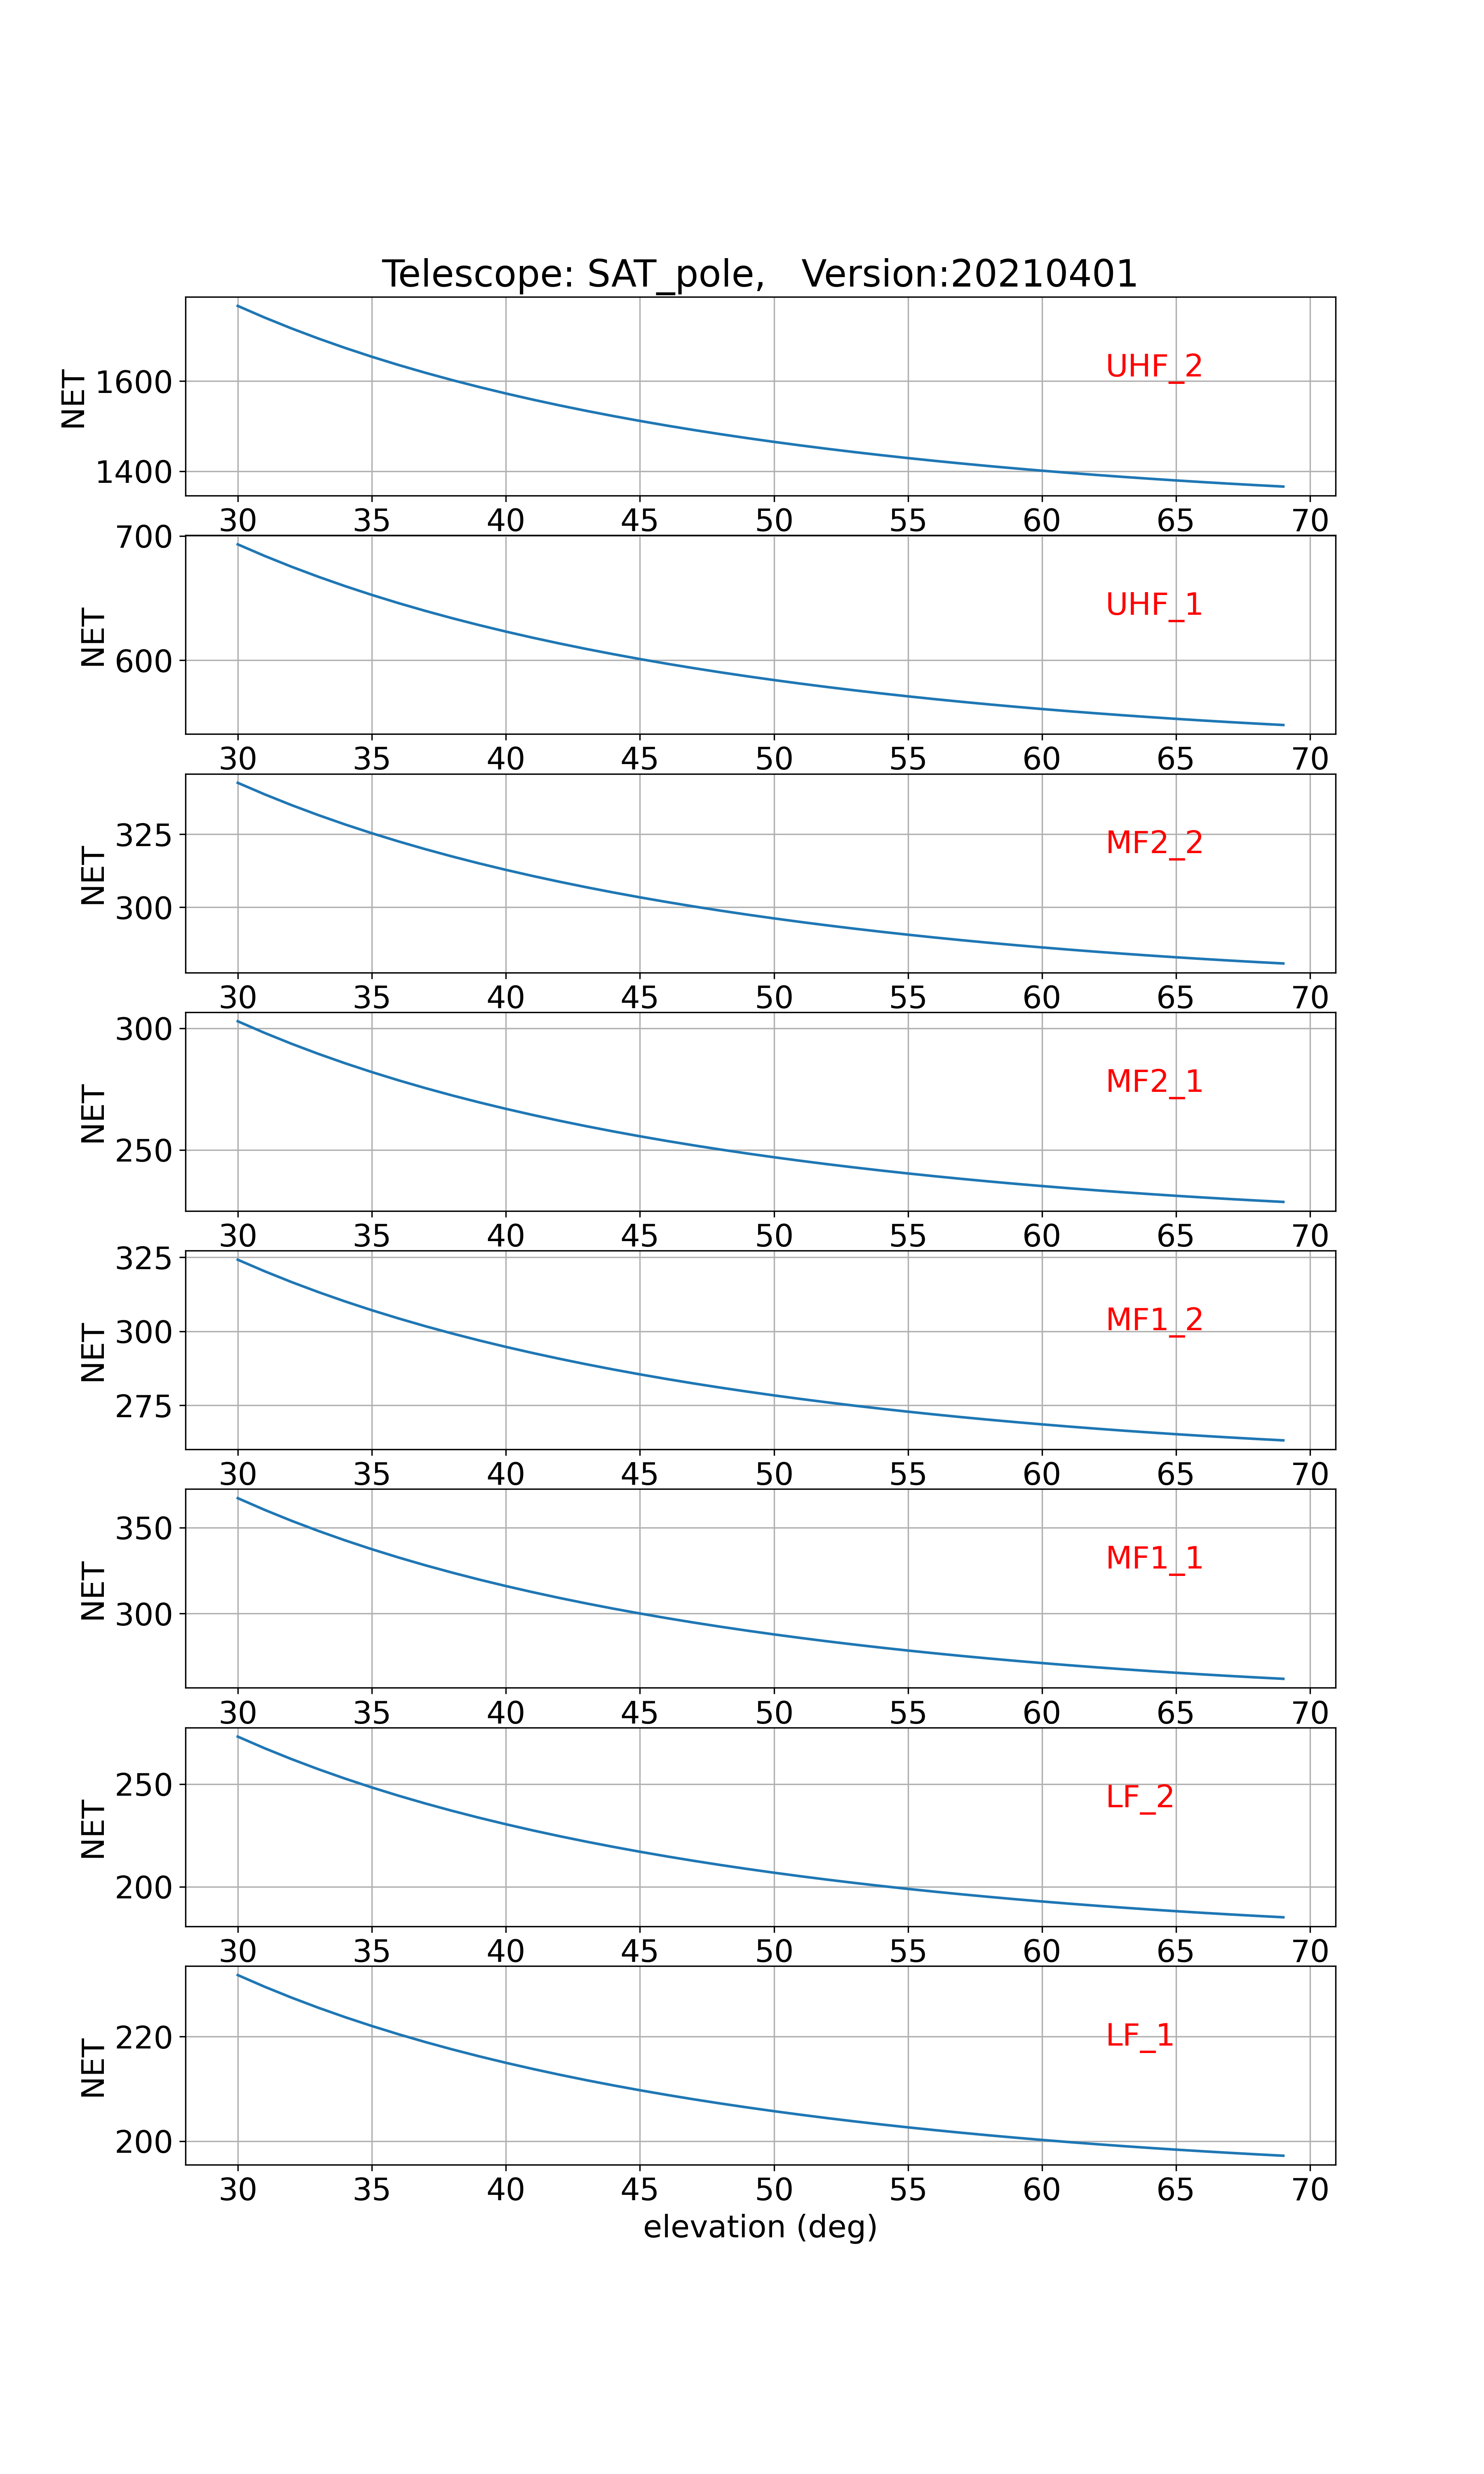
\includegraphics[width=0.33\textwidth]{plots/SAT_pole_20210401_NET_v_elevation.png}
            %\caption{}
        }
     %\vspace{-2\baselineskip}
     \caption{NET vs Elevation pointing}
     \label{fig:elev}
\end{figure} 


\begin{figure}[p]
         \centering
         \subfloat[Subfigure 1 list of figures text][CHLAT]{
             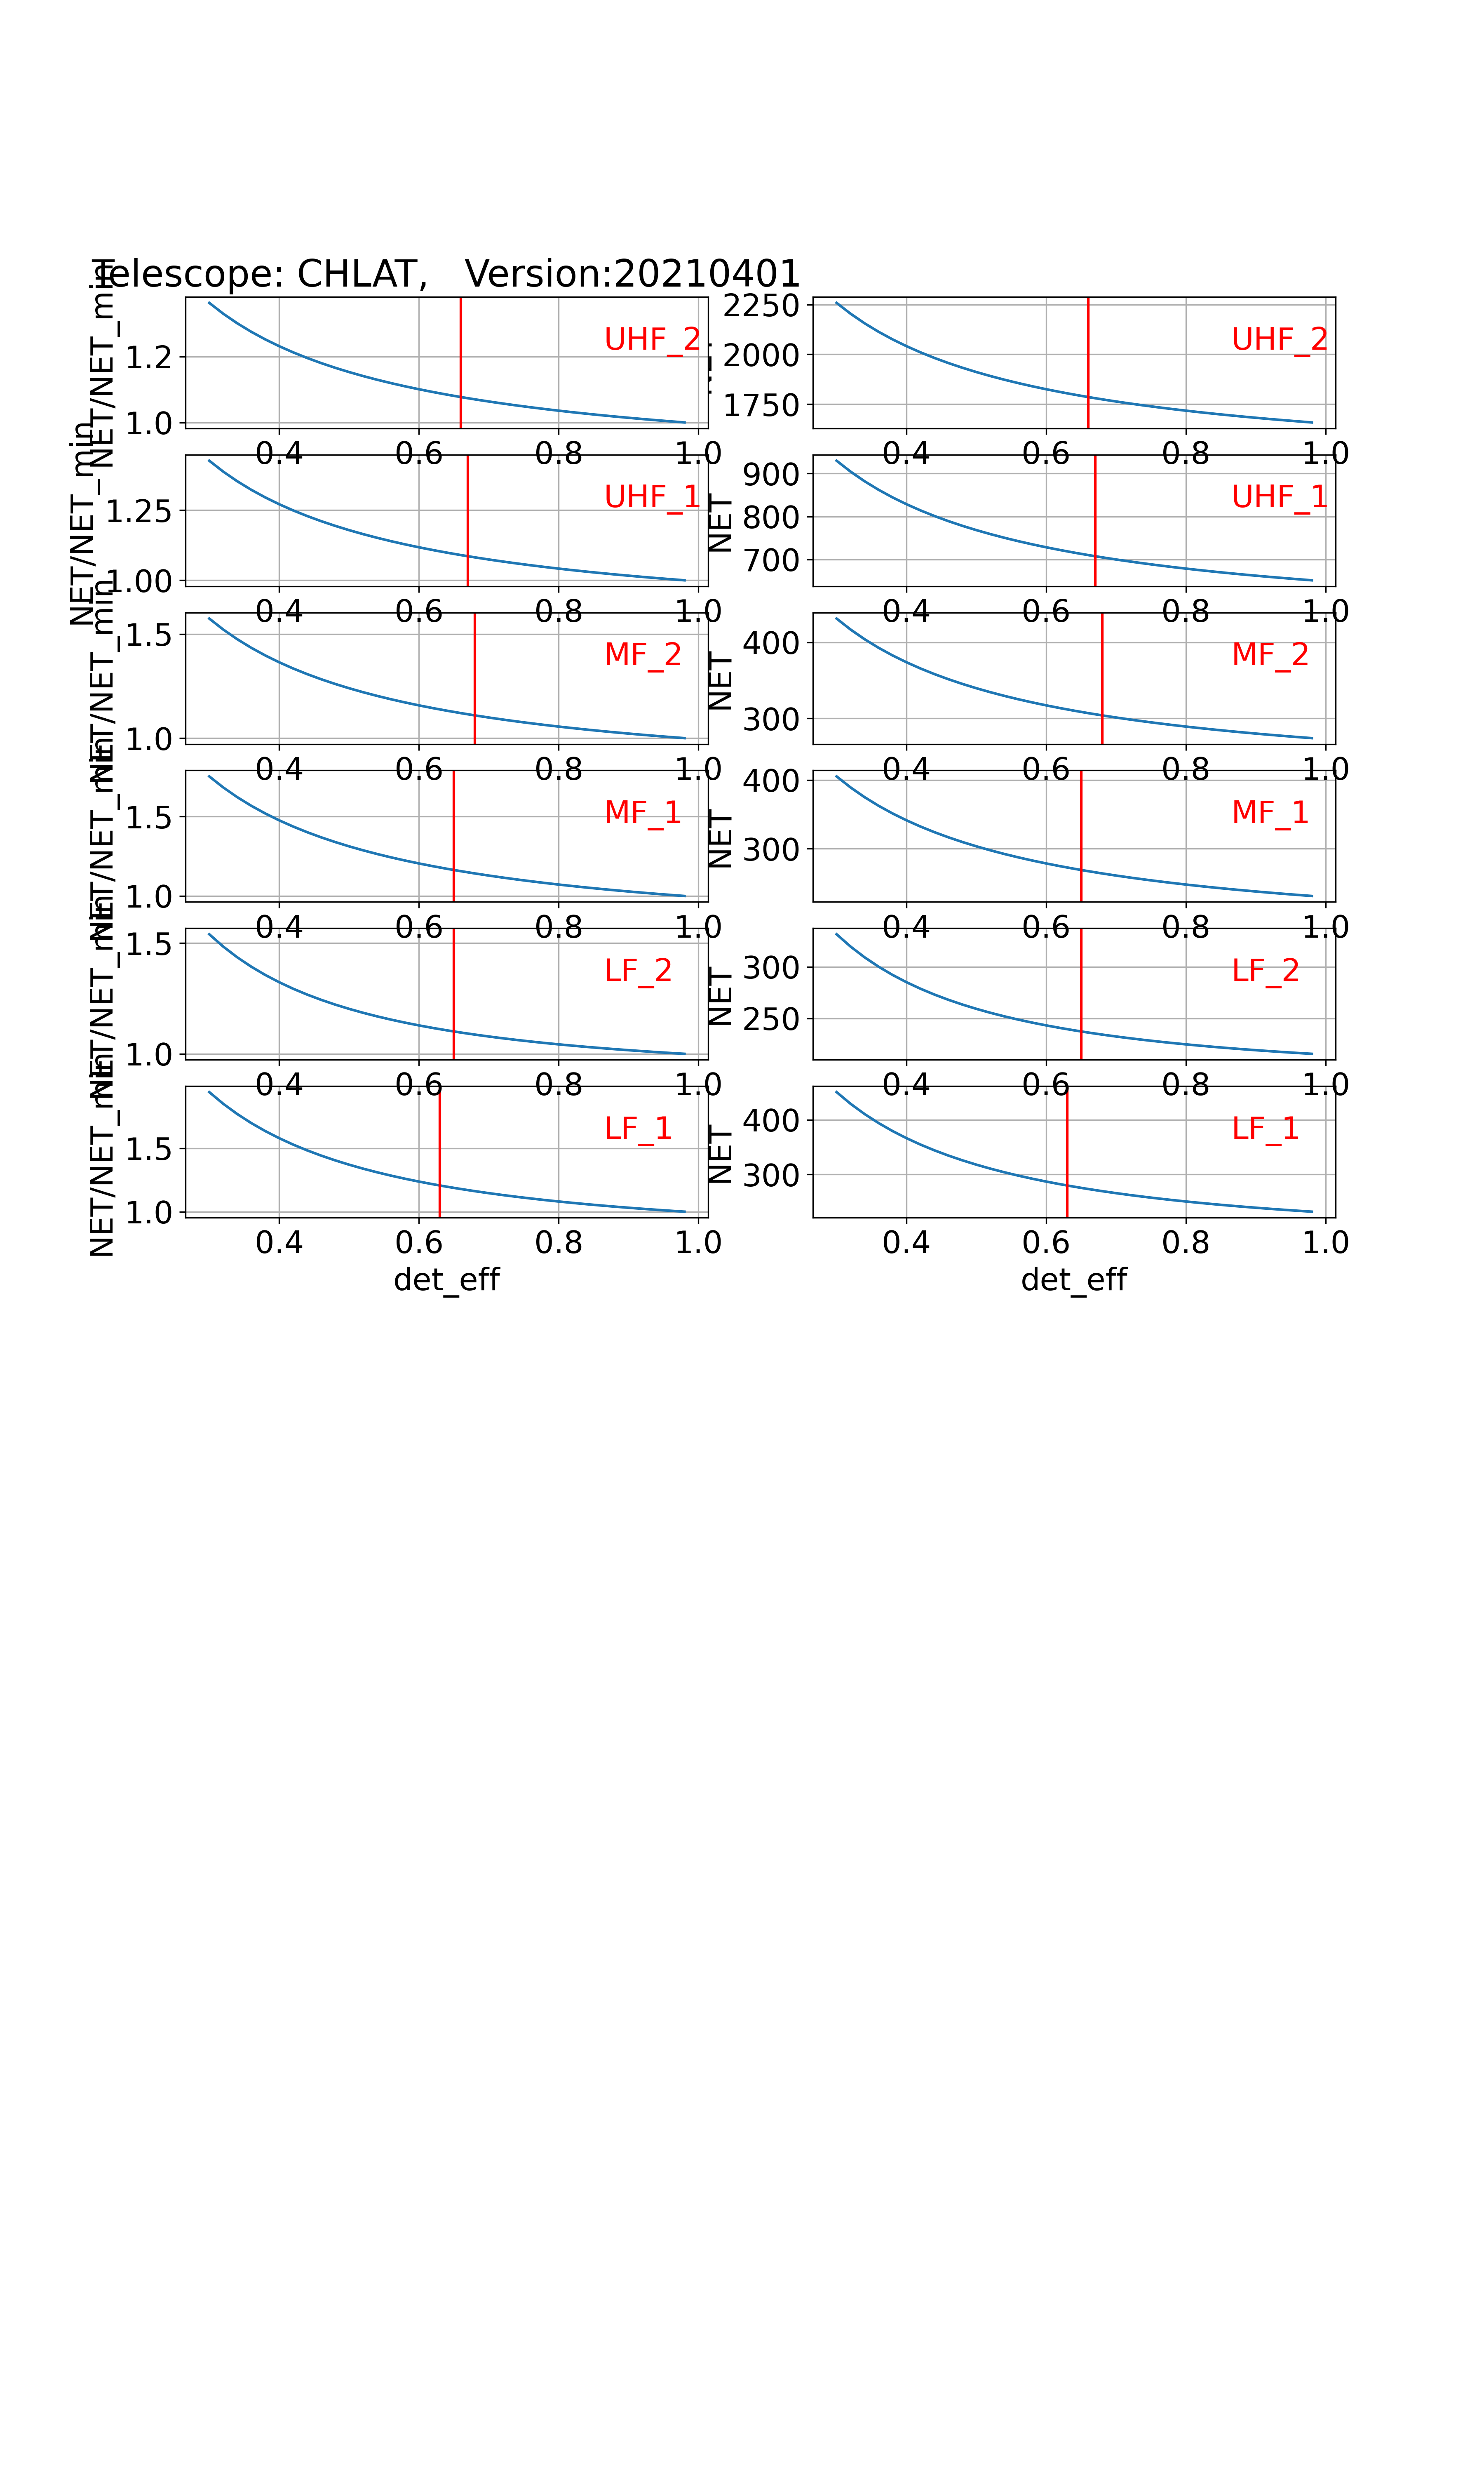
\includegraphics[width=0.33\textwidth]{plots/CHLAT_20210401_NET_v_det_eff.png}
             %\caption{}
         }
     %\hfil
        \subfloat[Subfigure 1 list of figures text][SPLAT]{
           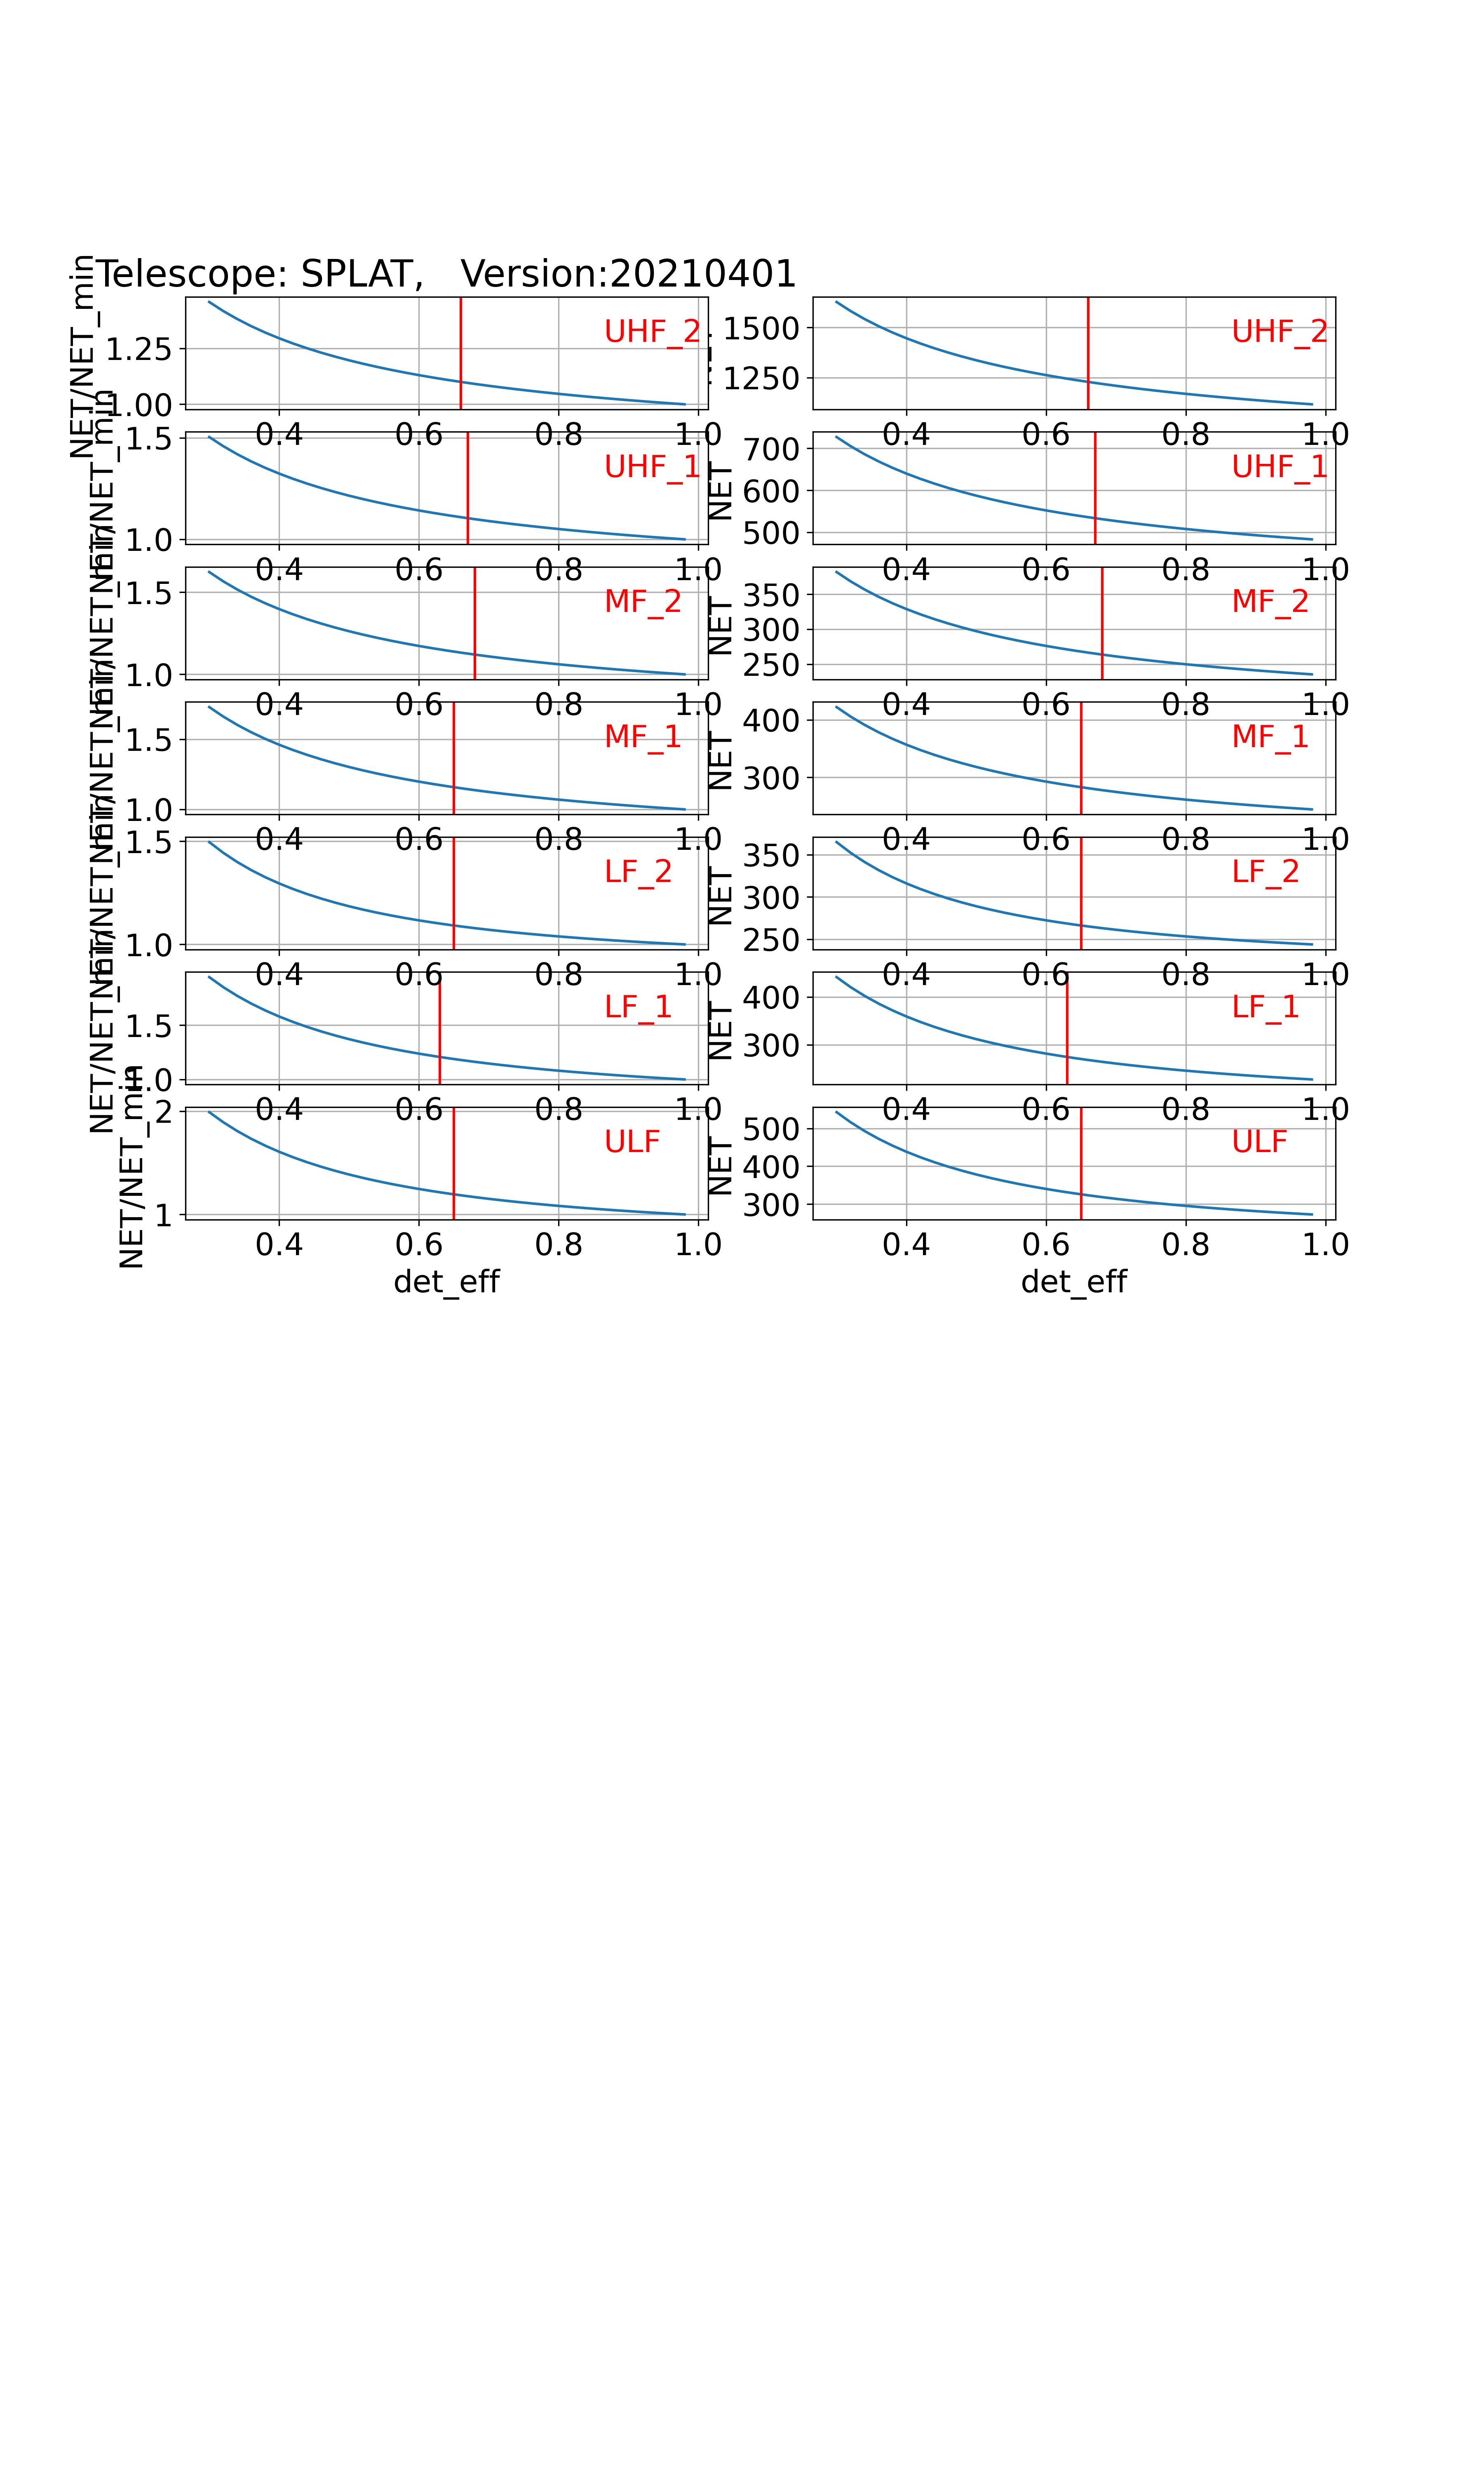
\includegraphics[width=0.33\textwidth]{plots/SPLAT_20210401_NET_v_det_eff.png}
           %\caption{}
        }    
        \subfloat[Subfigure 1 list of figures text][SAT]{
            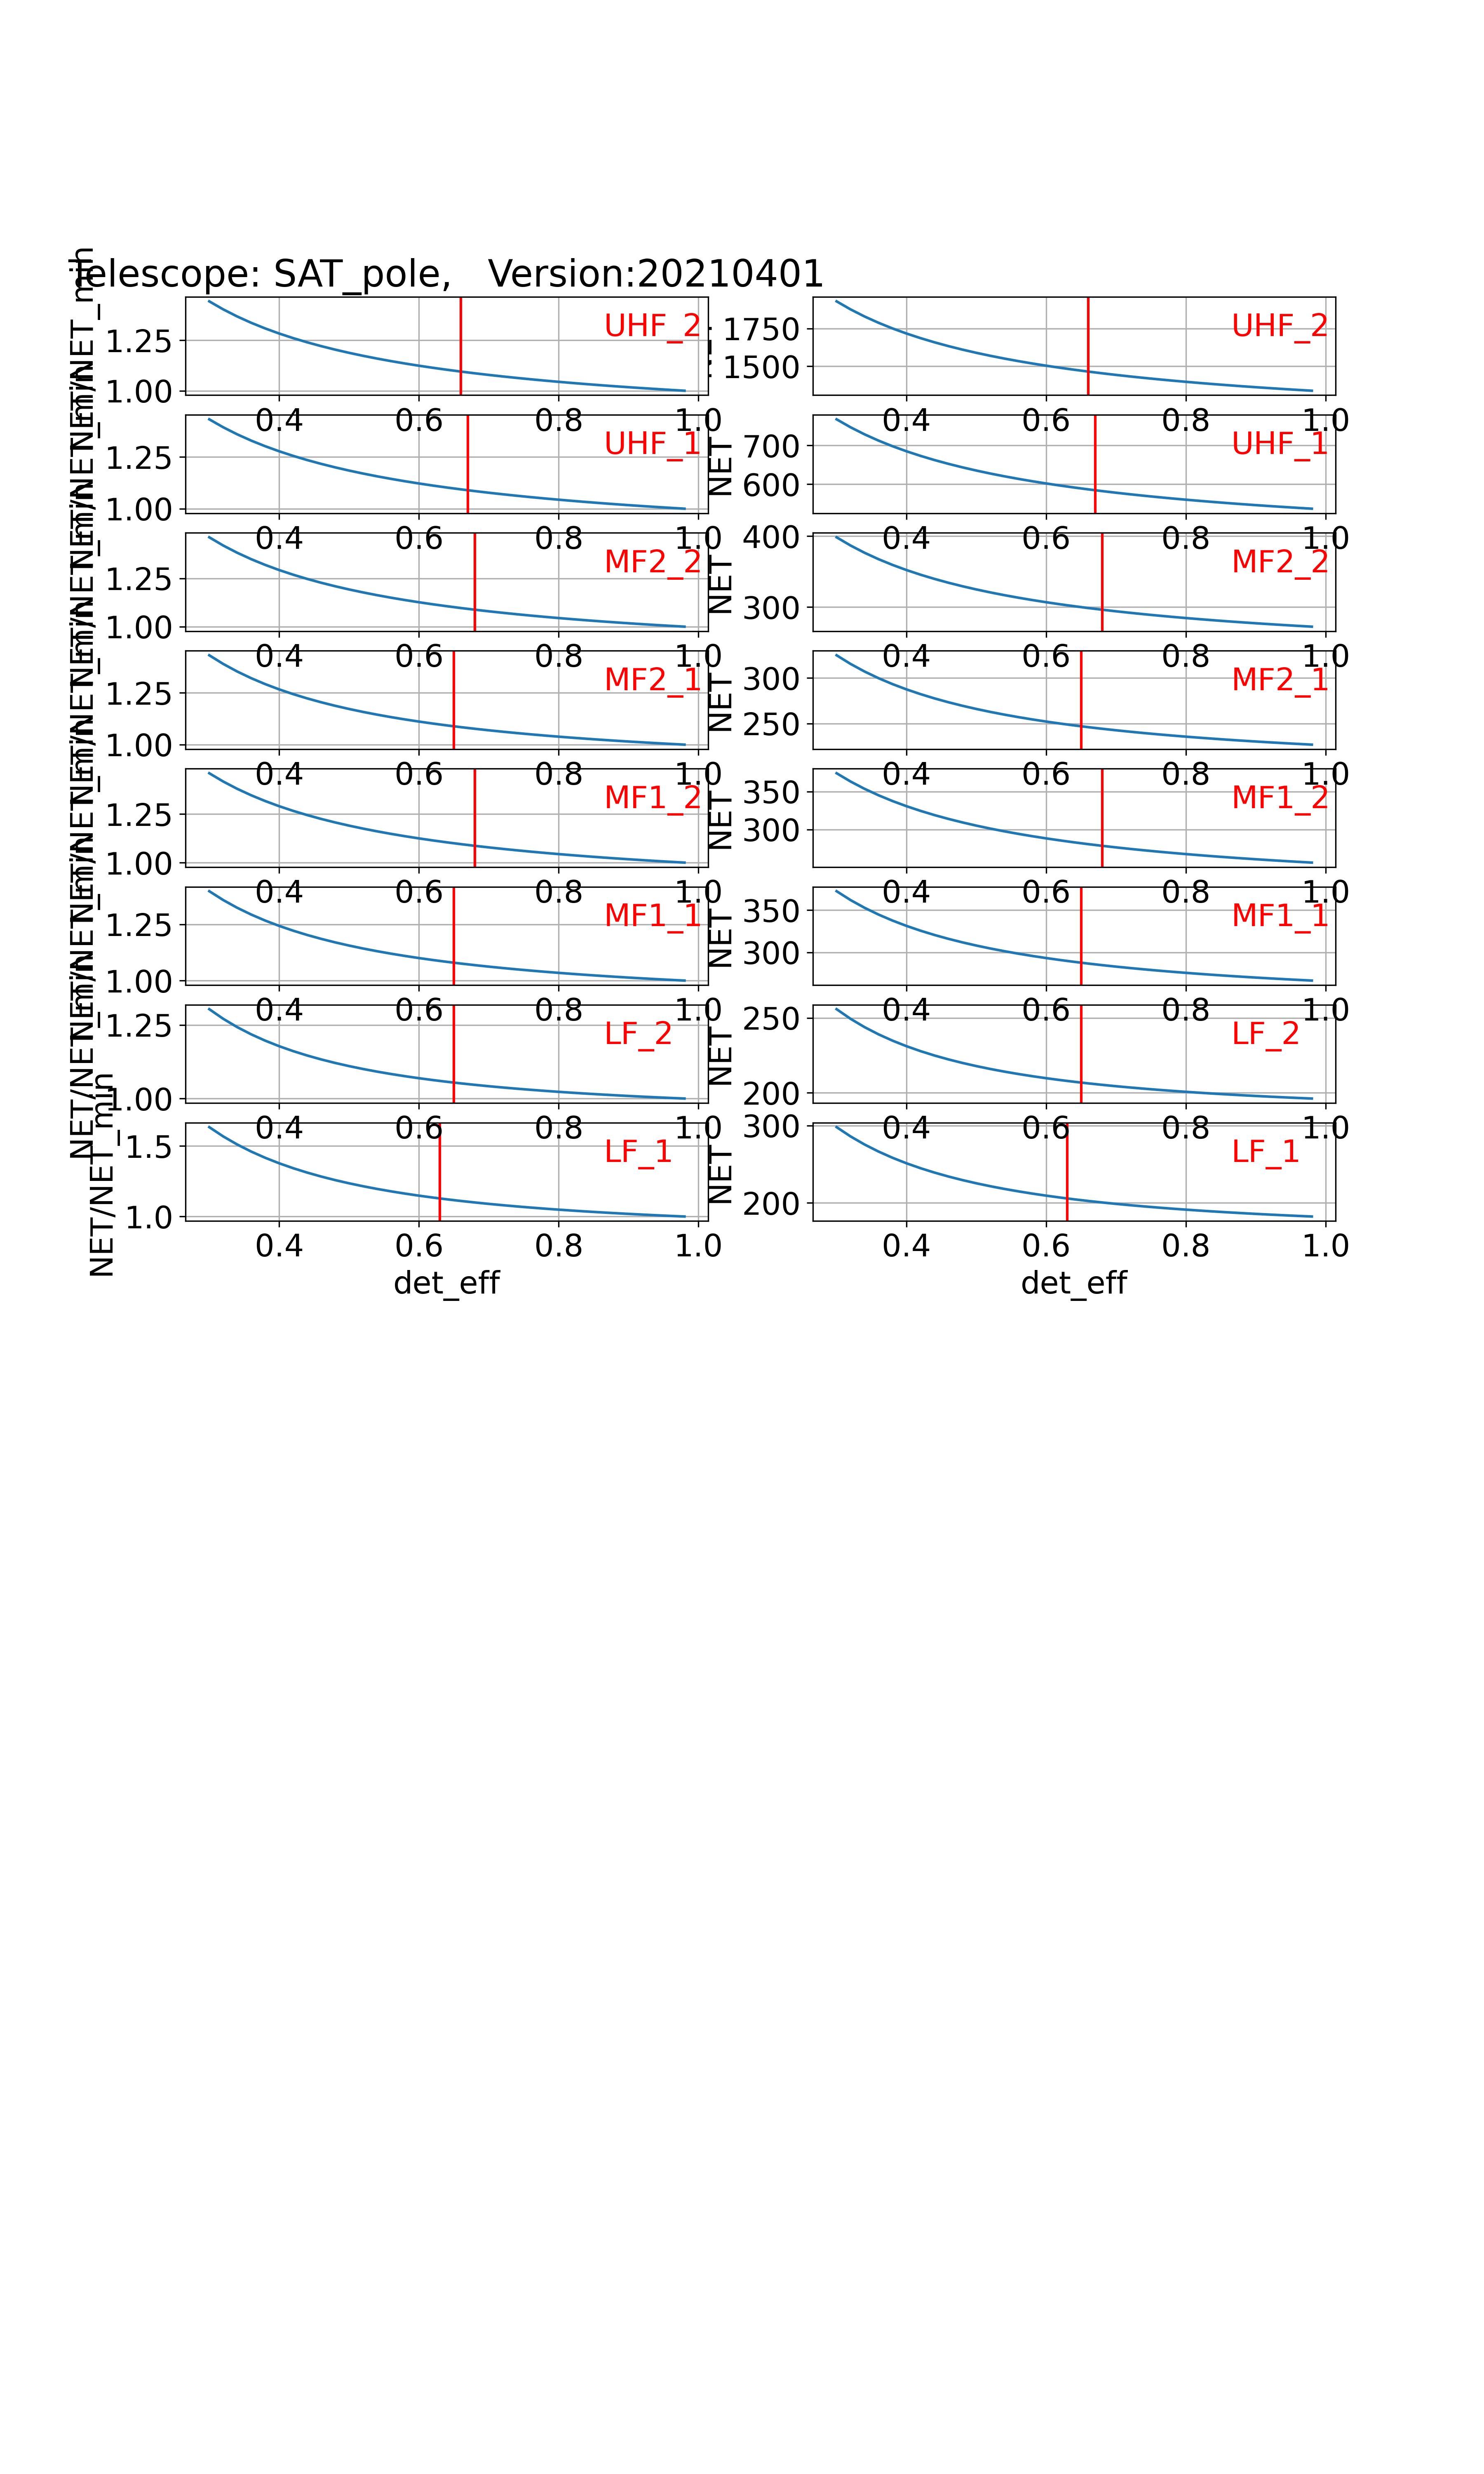
\includegraphics[width=0.33\textwidth]{plots/SAT_pole_20210401_NET_v_det_eff.png}
            %\caption{}
        }
     %\vspace{-2\baselineskip}
     \caption{NET vs Detector Efficiency}
     \label{fig:DetEff}
\end{figure} 





\end{document}